\documentclass{article}
\usepackage[utf8]{inputenc}
\title{vidio 2:A Two-Sample Test for Antetokounmpo's Free Throws}
\author{wbg231 }
\date{December 2022}
\newcommand{\R}{$\mathbb{R}$}
\newcommand{\B}{$\beta$}
\newcommand{\A}{$\alpha$}
\newcommand{\D}{\Delta}

\newcommand{\avector}[2]{(#1_2,\ldots,#1_{#2})}
\newcommand{\makedef}[2]{$\textbf{#1}$:#2 }
\usepackage{tikz,graphicx,hyperref,amsmath,amsfonts,amscd,amssymb,bm,cite,epsfig,epsf,url}

\begin{document}

\maketitle

\section{introduction}
\begin{itemize}
\item \href{https://www.youtube.com/watch?v=j3hTudQvM2o&list=PLBEf5mJtE6KuZ5NBQMuWIMsiOOrV9ibzm&index=79}{video link}
\item Antetokounmpo a really good player, but is not good at free throw shootings, he has a really long routine to get ready. the fans try to count during this routine, to throw him off
\item people were wondering if his free throw \% at home is different from his free throw \% at home
\item to do this we need a two sample test 
\subsection{hypothesis testing}
\item chose a conjecture 
\itme design a null hypothesis 
\item chose an appropriate test stat 
\item decide on significance level $\alpha$
\item gather data compute test stat 
\item compute p -value 
\item reject null if $p-val\leq \alpha$
\subsection{Antetokounmpo example}
\item our alternative hypothesis is that Antetokounmpo's free throw \% is different at home versus away
\item our null would thus be that his free throw percentage is the same at home and away
\item two sample test: data separated into two groups, our conjecture that the groups are form different distributions, null they are form the same distributions.
\subsection{test statistic}
\item test stat should be large if the null does not hold and should capture the structure of interest in our problem 
\item here we can take our test stat as $t_{data}=\frac{\textbf{shots made at home}}{\textbf{shots attempted at home}}- \frac{\textbf{shots made away}}{\textbf{shots attemtped away}}$
\item we can see that if he shoots better away then the test stat would not capture it well
\item data from 2021 nba finals (which we got after we thought of our hypothesis) $t_{data}=\frac{33}{44}-\frac{22}{41}=.236$ this seems like a big difference but can we be sure it is not random? 
\item no we need to compute the associated p-value
\subsection{p-value}
\item  p-value the probability of observing a larger or equal test stat under the null 
\subsection{two samples z test}
\item here we are choosing the two sample z test, but the idea extends to most two samples test
\item Data $\Tilde{x}_1..\Tilde{x}_n$ (these are Bernoulli equal to one if the shot is made) 
\item two groups A and B 
\item one tilled test stat $$\Tilde{t}_{1-tail}=\frac{1}{nA}\Sigma_{i\in A}\Tilde{x}_i-\frac{1}{nB}\Sigma_{i\in B}\Tilde{x}_i$$
\item our null hypothesis is that all data are iid Bernoulli with parameter $\theta_{null}$
\subsection{binomial distribution}
\item binomial random variable $\Tilde{a}$ with parameters n and $\theta$ $\approx$ Gaussian with mean $n\theta$ and variance $n\theta(1-\theta)$  (well approximated if they are independent and n is large)
\subsection{two sample z test }
\item null hypothesis all data are iid Bernoulli with parameter $\theta_{null}$
$$\Tilde{t}_{1-tail}=\frac{1}{nA}\Sigma_{i\in A}\Tilde{x}_i-\frac{1}{nB}\Sigma_{i\in B}\Tilde{x}_i$$
\item but we can see that $\Sigma_{i\in A}\Tilde{x}_i$ is a binomial with parameter $n_A$ and $\theta_{null}$
\item but as we know this 
is a sum of iid random Bernoulli variables and thus for a large n is approximately Gaussian with  $\Sigma_{i\in A}\Tilde{x}_i\sim \mathcal{N}(n_A\theta_{null},n_{A}\theta_{null}(1-\theta_{null}))$ 
\item then to take the sample mean we know it is just a Gaussian multiplied by a constant so we can take the sample mean as being distribution as $$\frac{1}{n_{A}}\Sigma_{i\in A}\Tilde{x}_i\approx \sim \mathcal{N}(\theta_{null},\frac{\theta_{null}(1-\theta_{null})}{n_{A}})$$ 
\item we can do the same thing for group B and see that (-1 times) there mean is $$-\frac{1}{n_{B}}\Sigma_{i\in B}\Tilde{x}_i\approx \sim \mathcal{N}(-\theta_{null},\frac{\theta_{null}(1-\theta_{null})}{n_{B}})$$ 
\item so we know that our test statistic is really the sum of these two things that are approximately Gaussian and we assumed are independent under the null hypothesis $$\Tilde{t}_{1-tail}=\frac{1}{nA}\Sigma_{i\in A}\Tilde{x}_i-\frac{1}{nB}\Sigma_{i\in B}\Tilde{x}_i\\\sim \approx\mathcal{N}(\theta_{null}-\theta_{null}, \frac{\theta_{null}(1-\theta_{null}}{n_A}-\frac{\theta_{null}(1-\theta_{null}}{n_B})$$ $$=\mathcal{N}(0, \theta_{null}(1-\theta_{null})(\frac{1}{n_A}+\frac{1}{n_B}))$$
\item it so now we have a distribution of our test stat under the null. 
\item there is a problem that we do not know $\theta_{null}$ in practice
\item we often just approximate $\theta_{null}$ over our whole dataset $$\theta_{null}\approx\frac{\textbf{number of 1's}}{n}$$
\subsection{back to free throw example}
\item $t_{data}=.236$
\item under the null we know  $\Tilde{t}_{1-tail}\approx\sim\mathcal{N}(0, \theta_{null}(1-\theta_{null})(\frac{1}{n_A}+\frac{1}{n_B}))=\sim\mathcal{N}(0, \theta_{null}(1-\theta_{null})(\frac{1}{n_A}+\frac{1}{n_B}))$ this has variance $.103$ from the data. 
\subsection{p value function}
\item so we are going $\Tilde{t}_{1-tail}\approx .103\Tilde{z}$
\item where $\Tilde{z}\sim \mathcal{N}(0,1)$ 
\item so $pv(t)=P(\Tilde{t}_{1-tai}\geq t)=P(\Tilde{z}\geq \frac{t}{.103}$ 
\section{two tailed test}
\item we just did a 1-tailed test that is we assumed that he shoots worse away, but this will not catch if he shoots better away. (which would still mean the two distributions are different)
\item for cases where we want to see if the distributions are different in a smaller or larger way we can say $\Tilde{t}_{2-tail}=|\frac{1}{n_A}\Sigma_{i\in A}\Tilde{x}_{i}-\frac{1}{n_{B}}\Sigma_{i\in B}\Tilde{x}_i|$
\item 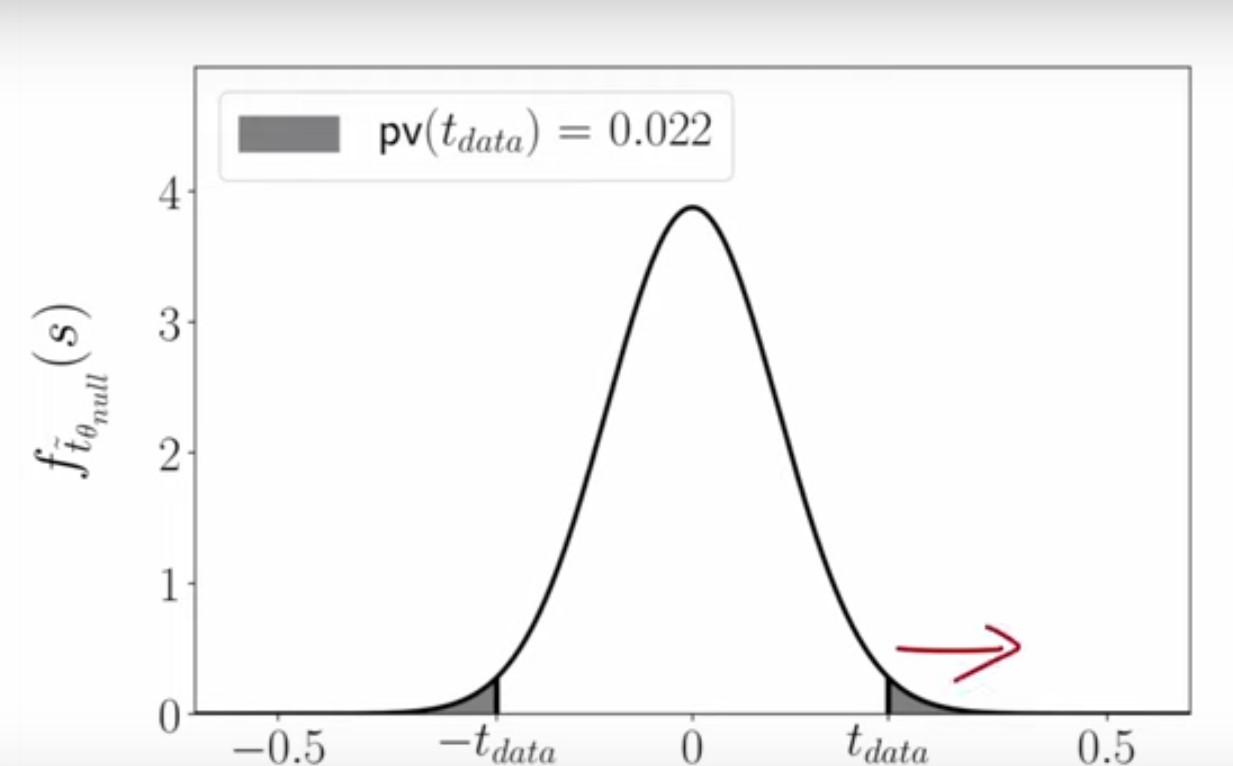
\includegraphics[width=10cm]{notes/week_6/vidio 2: A Two-Sample Test for Antetokounmpo's Free Throws/immages/v1_3.jpg}
\item so graphically this captures both sides of the distribution 
\item that would make the p-value double what it was before, and makes it easier to reject the null
\subsection{statistical difference }
\item we reject the null when $p-value\leq \alpha$
\item this guarantees that the probability of false positive $\leq \alpha$
\item so in this case we see we reject the null. so it is unlikely for this data to be observed under the null due to random chance alone 
\item \textbf{but this does not mean we can make any casual statements about why this happened }
\item here we do not have randomization so there could be confounding factors that caused this difference, like we are not controlling for how tired he is,how good the other team is etc. 
\item in order to ensure we can have a casual interpretation we need the treatment to be independent of the casual outcome and that has to happen with randomization. 
\end{itemize}
\end{document}
